\section{Add a new client}(fields marked  with * have to be filled in)\\
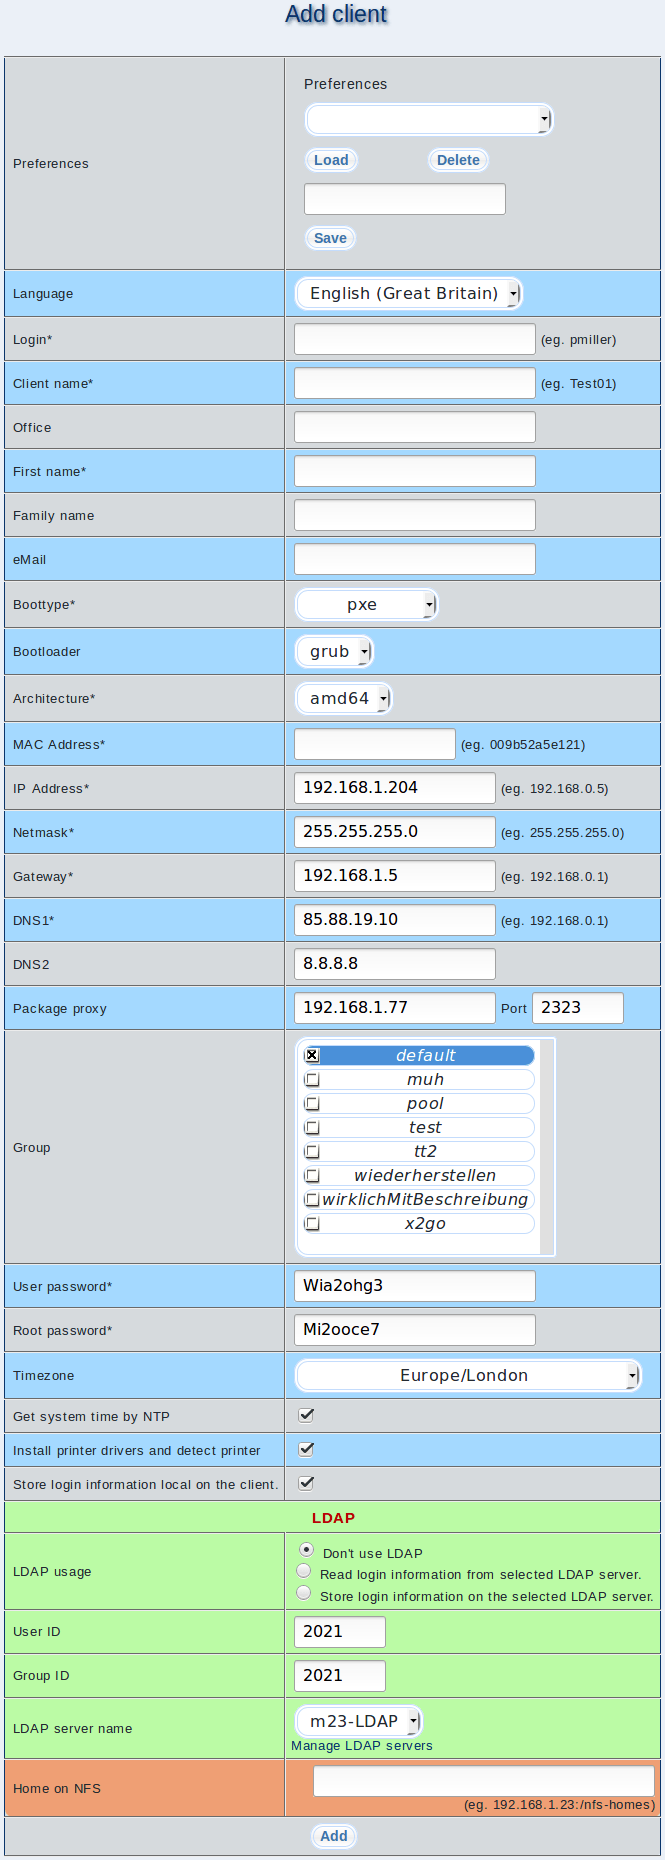
\includegraphics[scale=0.4]{/mdk/doc/manual/screenshots/en/client_add.png} \\
\begin{itemize}
\item \textbf{Preferences:} You can select saved preferences and load or delete them. If you want to save your current client's settings, enter a name for your preference and click on \textit{"Save"}.\\
\item \textbf{Language:} You can choose the language for your m23 client. This language setting is used for the keyboard, desktop and console.\\
\item \textbf{Login:} The name for logging into the client.\\
\item \textbf{Client name:} Is the name of your client, it should be unique.\\
\item \textbf{Office:} Here you can enter the location of the client (room number, etc.).\\
\item \textbf{First name:} The first name of the user\\
\item \textbf{Family name:} The family name of the user\\
\item \textbf{eMail:} eMail address of the user\\
\item \textbf{Boottype:} Boot standard for booting your clients over the network (Hint: Please read the following page, if you want to use m23 with an existing DHCP server: externalDHCP)\\
\item \textbf{Bootloader:} Choose the boot loader/boot manager for starting the Linux kernel and possibly already installed other operating systems. You can choose between LILO (LInux LOader) and GRUB (GRand Unified Bootloader).\subsection{Hint}
Clients installed with m23 0.6.4 or higher secure the bootparameters against editing via the bootmanager. The networkboot password is needed to unlock the editing function of the bootmanager. The password can be found in the control center for the specific client under \textit{"Client direct connection"}.\\
\item \textbf{Architecture:} Choose if you want to install 32 or 64 bit software on the client. Please check the hint on the bottom of the page.\\
\item \textbf{MAC Address:} MAC address of the client network card (e.g. 00:D0:B7:23:86:5C)\\
\item \textbf{IP Address:} IP address of the client (e.g. 192.168.1.23)\\
\item \textbf{Netmask:} Networkmask of your network (e.g. 255.255.255.0)\\
\item \textbf{Gateway:} Gateway IP for internet connections\\
\item \textbf{DNS1:} IP address for the first DNS server\\
\item \textbf{DNS2 (optional):} IP address for the second DNS server\\
\item \textbf{Package proxy:} The client tries to fetch its software packages from the denoted proxy server IP. In the normal case this is the IP of the m23 server, but you can choose the IP of another proxy server instead. If you leave this field empty the client will download the software packages directly from the internet. Enter the port address of the proxy server, please. The proxy on the m23 server uses port 2323. When the \textit{"Add client"} dialog is opened the m23 server is preselected as proxy server.\\
\item \textbf{Group (optional):} Group the client belongs to\\
\item \textbf{User password:} This is the user password used for the first log in. It is automatically generated by m23 with 6 characters, but you can enter your own password.\\
\item \textbf{Root password:} This is the root password. It is automatically generated by m23 with 6 characters, but you can enter your own password.\\
\item \textbf{Timezone:} You can choose the time zone that will be used for your client here.\\
\item \textbf{Get system time by NTP:} Set this option if the client should get its system time over the internet.\\
\item \textbf{Install printer drivers and detect printer:} Choose this option to install printer drivers and autodetect attached printers.\\
\item \textbf{Store login information local on the client.:}Check this option if you want a local account for the user on the client.\\
\item \textbf{Don't user LDAP}: If you want to use the local user authentification only you should select \textit{"Don't user LDAP"}. \\
\item \textbf{Read login information from selected LDAP server.}: Existing user authetification entries in a LDAP server can be used for client login. This is enabled with \textit{"Read login information from selected LDAP server."}.\\
\item \textbf{Store login information on the selected LDAP server.}: New login information can be written to a LDAP server and used afterwards for client login. Choose \textit{"Store login information on the selected LDAP server."}. This option requires a LDAP server with "full access".\\
\item \textbf{User ID, Group ID}: You have to enter the \textit{"User ID"} and \textit{"Group ID"} for the user account. This is especially important if you want to use the "Home on NFS" feature.\\
\item \textbf{LDAP server name}: The last step for using LDAP is to choose a LDAP server under  \textit{"LDAP server name"}. If your desired LDAP server is not available you can add it with a click on \textit{"Manage LDAP servers"}.\\
\item \textbf{Home on NFS:} This option enables the saving of the home directories on a central NFS server. It may be usefull (in combination with LDAP) because you can access the user data from every client. Enter the hostname or IP of your NFS server followed by the path to store the home directories in to activate NFS. E.g \\
\begin{verbatim}
192.168.1.42/nfs/home
\end{verbatim}
.\\
\end{itemize}
\subsection{Additional information:}
After adding a new client, the client will boot over the network and runs through a hardware detection sequence. Hardware data (hard disk size, partitions etc.) will be sent to the server. When the data transfer is finished the client will change its status to \textit{"yellow"}. You can setup your client now. To setup your client click on \textit{"Clients"} $\rightarrow$ \textit{"Setup"} in the menu.\\
\subsection{Hint for computer architectures}
m23 supports 32 and 64 bit systems natively. A 32 bit distribution can be installed on a 64 bit computer, but not vice versa. You should choose \textit{"amd64"} to use the full potential of a 64 bit CPU. Not only AMD's 64 bit CPUs, but also Intel's fall under the category of \textit{"amd64"}. Some of the supported 64 bit CPUs are Intel Pentium D, Pentium Extreme Edition, Celeron D and Core 2 and the AMD CPUs Sempron, Athlon 64, Athlon X2 and Phenom.\\
